% =============================================================================
% StructureTower_TopologyBridge.tex
% LuaLaTeX document — Lean 4 形式化の数学的解説
% =============================================================================
\documentclass[a4paper,11pt]{ltjsarticle}

% --- Core packages ---
\usepackage{luatexja-fontspec}
\usepackage{amsmath,amssymb,amsthm}
\usepackage{mathtools}
\usepackage{tikz-cd}
\usepackage{enumitem}
\usepackage{hyperref}
\usepackage{cleveref}
\usepackage{tcolorbox}
\usepackage{listings}
\usepackage{xcolor}
\usepackage{geometry}
\usepackage{fancyhdr}
\usepackage{float}
\usepackage{booktabs}
\usepackage{array}
\usepackage{multirow}

\tcbuselibrary{skins,breakable}
\usetikzlibrary{cd,arrows.meta,positioning,fit,backgrounds,decorations.pathreplacing}

% --- Page geometry ---
\geometry{margin=2.5cm, top=3cm, bottom=3cm}

% --- Fonts ---
\setmainjfont{Harano Aji Mincho}
\setsansjfont{Harano Aji Gothic}

% --- Colors ---
\definecolor{leanblue}{HTML}{2563EB}
\definecolor{leanbg}{HTML}{F8FAFC}
\definecolor{leancomment}{HTML}{6B7280}
\definecolor{leankeyword}{HTML}{7C3AED}
\definecolor{leanstring}{HTML}{059669}
\definecolor{accentcolor}{HTML}{1E40AF}
\definecolor{theoremcolor}{HTML}{EFF6FF}
\definecolor{definitioncolor}{HTML}{F0FDF4}
\definecolor{remarkcolor}{HTML}{FFF7ED}

% --- Hyperref ---
\hypersetup{
  colorlinks=true,
  linkcolor=accentcolor,
  urlcolor=leanblue,
  citecolor=accentcolor,
  pdftitle={StructureTower による位相空間ブリッジ},
  pdfauthor={su},
}

% --- Theorem environments ---
\theoremstyle{definition}
\newtheorem{definition}{定義}[section]
\newtheorem{example}[definition]{例}

\theoremstyle{plain}
\newtheorem{theorem}[definition]{定理}
\newtheorem{lemma}[definition]{補題}
\newtheorem{proposition}[definition]{命題}
\newtheorem{corollary}[definition]{系}

\theoremstyle{remark}
\newtheorem{remark}[definition]{注意}

% --- Lean code environment ---
\lstdefinelanguage{lean4}{
  morekeywords={def,theorem,lemma,example,instance,class,structure,
    where,let,in,do,if,then,else,match,with,fun,return,
    import,open,namespace,section,end,variable,
    inductive,abbrev,noncomputable,private,protected,
    sorry,admit,have,show,suffices,calc,by,exact,
    apply,intro,intros,constructor,cases,induction,
    simp,rw,rfl,ext,ring,linarith,omega,norm_num,
    decide,trivial,assumption,contradiction,
    Type,Prop,Sort,Set,true,false,omit,
    rcases,obtain,refine,exact,change,
    attribute,deriving},
  sensitive=true,
  morecomment=[l]{--},
  morecomment=[n]{/-}{-/},
  morestring=[b]",
}

\lstnewenvironment{leancode}[1][]{%
  \lstset{
    language=lean4,
    basicstyle=\ttfamily\small,
    keywordstyle=\color{leankeyword}\bfseries,
    commentstyle=\color{leancomment}\itshape,
    stringstyle=\color{leanstring},
    backgroundcolor=\color{leanbg},
    frame=single,
    rulecolor=\color{leanblue!30},
    framesep=8pt,
    xleftmargin=12pt,
    xrightmargin=12pt,
    breaklines=true,
    breakatwhitespace=true,
    showstringspaces=false,
    tabsize=2,
    captionpos=b,
    numbers=left,
    numberstyle=\tiny\color{leancomment},
    numbersep=8pt,
    aboveskip=1em,
    belowskip=1em,
    #1
  }%
}{}

% --- Tcolorbox styles ---
\newtcolorbox{proofstrategy}{
  colback=remarkcolor,
  colframe=orange!60!black,
  title={\textbf{証明戦略}},
  fonttitle=\sffamily,
  boxrule=0.5pt,
  arc=3pt,
}

\newtcolorbox{mathinsight}{
  colback=theoremcolor,
  colframe=accentcolor,
  title={\textbf{数学的洞察}},
  fonttitle=\sffamily,
  boxrule=0.5pt,
  arc=3pt,
}

\newtcolorbox{analogybox}{
  colback=definitioncolor,
  colframe=green!50!black,
  title={\textbf{3分野の対応}},
  fonttitle=\sffamily,
  boxrule=0.5pt,
  arc=3pt,
}

% --- Header/Footer ---
\pagestyle{fancy}
\fancyhf{}
\renewcommand{\headrulewidth}{0.4pt}
\fancyhead[L]{\small\sffamily\nouppercase{\leftmark}}
\fancyhead[R]{\small\sffamily StructureTower --- 位相空間ブリッジ}
\fancyfoot[C]{\thepage}

% --- Math macros ---
\newcommand{\Nbd}{\mathcal{N}}
\newcommand{\Opens}{\mathcal{O}}
\newcommand{\Filt}{\mathsf{Filt}}
\newcommand{\Tower}{\mathsf{Tower}}
\newcommand{\level}{\mathrm{level}}
\newcommand{\NatIncl}{\mathrm{NatInclusion}}
\newcommand{\reindex}{\mathrm{reindex}}
\newcommand{\iInf}{\mathrm{iInf}}
\newcommand{\iSup}{\mathrm{iSup}}
\newcommand{\inte}{\mathrm{int}}
% Definitional connectives
\newcommand{\coloniff}{\mathrel{:\!\!\Longleftrightarrow}}
\newcommand{\coloniss}{\mathrel{:=}}

% =============================================================================
\begin{document}
% =============================================================================

% --- Title ---
\title{%
  {\LARGE\sffamily\bfseries StructureTower による位相空間ブリッジ}\\[0.5em]
  {\large\sffamily フィルター・開被覆・内部作用素の統一的形式化}\\[0.3em]
  {\normalsize\sffamily Lean 4 / Mathlib4 形式化とその数学的解説}%
}
\author{su}
\date{\today}
\maketitle
\thispagestyle{empty}

% --- AI Disclosure ---
\begin{center}
\small
\textit{AI assistance disclosure:}\\
Lean ソースコードは Claude (Anthropic) で骨格を生成し、
Codex (OpenAI) で修正した。\\
\TeX\ 文書は Claude Code (Anthropic) で生成した。\\
著者による加筆・修正は行っていない。\\
内容の正確性は保証されず、誤りがあれば著者の責任である。
\end{center}

\vspace{1em}

% --- Abstract ---
\begin{abstract}
本稿は Lean~4 / Mathlib4 で形式化された \texttt{StructureTower\_TopologyBridge.lean}
の数学的内容を解説する。
\emph{StructureTower} とは、前順序集合 $(\iota, \leq)$ を添字集合として
$\alpha$ の部分集合の単調族 $\level\colon \iota \to \mathcal{P}(\alpha)$
を与える抽象的な構造である。
本稿では、この統一的な API が代数(フィルター)・位相(開集合・内部)・
位相群(近傍系)の三分野にわたってそれぞれ自然なタワー構造を与え、
互いに比較可能であることを形式的に示す。
具体的には、フィルタータワー($\mathsf{filterTower}$)、
開被覆タワー($\mathsf{openCoverTower}$)、
内部タワー($\mathsf{interiorTower}$)、
および位相群の単位元近傍タワー($\mathsf{unitNeighborhoodTower}$)を構築し、
$\NatIncl$・$\reindex$・$\iInf$ の三操作がそれぞれの分野で
何を意味するかを定理として明示する。
\end{abstract}

\tableofcontents
\newpage

% =============================================================================
\section{序論}
% =============================================================================

数学の様々な分野において「段階的な構造」が現れる:
代数では環のフィルトレーション(部分群 $G_0 \supseteq G_1 \supseteq \cdots$)、
位相では点の近傍基(より精密な近傍の族)、
解析では関数の収束の度合い(一様収束・各点収束など)。
これらは表面的には異なる文脈に属するが、実は共通の「前順序で添字付けられた
単調集合族」という骨格を持つ。

本稿の中心的なアイデアは \textbf{StructureTower} という抽象構造を通じて
こうした共通性を Lean~4 の型検査器に認証させることにある。
一度この共通 API を確立すれば、代数・位相・位相群で証明した定理が
同じ操作体系の下で比較・流用できる。

\begin{figure}[H]
\centering
\begin{tikzcd}[column sep=3.5em, row sep=3em]
  & \text{StructureTower} \arrow[dl, "\text{フィルター}"'] \arrow[d, "\text{開集合}"] \arrow[dr, "\text{位相群}"] & \\
  \mathsf{filterTower} & \mathsf{openCoverTower} \arrow[d, phantom, "\cong" description] & \mathsf{unitNeighborhoodTower} \\
  & \mathsf{interiorTower} &
\end{tikzcd}
\caption{StructureTower の三分野への展開}
\label{fig:overview}
\end{figure}

本稿の構成は次のとおりである。
\S\ref{sec:core} で StructureTower のコア定義と基本操作を述べ、
\S\ref{sec:filter} でフィルタータワーを、
\S\ref{sec:opencover} で開被覆タワーを、
\S\ref{sec:interior} で内部タワーをそれぞれ構築する。
\S\ref{sec:comparison} で三分野を横断する比較定理を与え、
\S\ref{sec:topgroup} で位相群のフィルトレーション的側面を論じ、
\S\ref{sec:conclusion} でまとめる。

% =============================================================================
\section{コア定義: StructureTower}
\label{sec:core}
% =============================================================================

\subsection{定義}

\begin{definition}[StructureTower]
\label{def:structure-tower}
前順序集合 $(\iota, \leq)$ と型 $\alpha$ に対して,
\emph{StructureTower} とは次のデータからなる:
\begin{itemize}
  \item 写像 $\level\colon \iota \to \mathcal{P}(\alpha)$(各添字に部分集合を対応させる)
  \item 単調性の証明: $i \leq j \Rightarrow \level(i) \subseteq \level(j)$
\end{itemize}
すなわち,StructureTower は前順序集合 $(\iota, \leq)$ から
冪集合束 $(\mathcal{P}(\alpha), \subseteq)$ への単調写像である。
\end{definition}

\begin{figure}[H]
\centering
\begin{tikzcd}[column sep=4em, row sep=3em]
  \cdots \arrow[r, "{\leq}"] & i \arrow[r, "{\leq}"] \arrow[d, mapsto, "\level"] & j \arrow[r, "{\leq}"] \arrow[d, mapsto, "\level"] & \cdots \\
  \cdots & \level(i) \arrow[r, hook, "\subseteq"] & \level(j) & \cdots
\end{tikzcd}
\caption{StructureTower: 前順序に沿って部分集合が単調増加する}
\label{fig:tower-monotone}
\end{figure}

Lean~4 での定義は次のとおりである。

\begin{leancode}
@[ext]
structure StructureTower (i a : Type*) [Preorder i] : Type _ where
  level          : i -> Set a
  monotone_level : forall (i j : i), i <= j -> level i ⊆ level j
\end{leancode}

\begin{remark}
\texttt{@[ext]} 属性により,\texttt{StructureTower.ext} 補題が自動生成される:
二つのタワーはすべての添字で同じ level を持てば等しい。
\end{remark}

\subsection{基本操作}

StructureTower の上には次の三つの基本操作が定義される。

\begin{definition}[NatInclusion(自然な包含)]
\label{def:nat-inclusion}
二つのタワー $T_1, T_2 : \Tower(\iota, \alpha)$ に対して,
\[
  \NatIncl(T_1, T_2) \;\coloniff\; \forall i \in \iota,\; T_1.\level(i) \subseteq T_2.\level(i).
\]
これは各レベルでの点別包含関係である。
\end{definition}

\begin{definition}[reindex(再添字化)]
\label{def:reindex}
単調写像 $f\colon (\iota, \leq_\iota) \to (\kappa, \leq_\kappa)$ と
タワー $T : \Tower(\kappa, \alpha)$ に対して,
\[
  (\reindex\; f\; T).\level(i) \coloniss T.\level(f(i)).
\]
これは $f$ に沿った引き戻し(pullback)である。
\end{definition}

\begin{definition}[iInf・iSup(族の交叉・合併)]
\label{def:iinf-isup}
タワーの族 $\{T_s\}_{s \in \sigma}$ に対して,
\begin{align*}
  (\iInf_{s} T_s).\level(i) &\coloniss \bigcap_{s \in \sigma} T_s.\level(i), \\
  (\iSup_{s}  T_s).\level(i) &\coloniss \bigcup_{s \in \sigma} T_s.\level(i).
\end{align*}
単調性は交叉・合併の単調性から従う。
\end{definition}

\begin{figure}[H]
\centering
\begin{tikzcd}[column sep=4em, row sep=3.5em]
  (\iota, \leq_\iota)
    \arrow[r, "f", "\text{単調}"']
    \arrow[dr, "(\reindex\,f\,T).\level"', bend right=20]
  & (\kappa, \leq_\kappa)
    \arrow[d, "T.\level"]
  \\
  & (\mathcal{P}(\alpha), \subseteq)
\end{tikzcd}
\caption{reindex は単調写像に沿った引き戻し}
\label{fig:reindex}
\end{figure}

\begin{leancode}
def NatInclusion (T1 T2 : StructureTower i a) : Prop :=
  forall i, T1.level i ⊆ T2.level i

def reindex {k : Type*} [Preorder k] (f : i -> k) (hf : Monotone f)
    (T : StructureTower k a) : StructureTower i a where
  level i        := T.level (f i)
  monotone_level := fun _i _j hij => T.monotone_level (hf hij)

def iInf {s : Type*} (T : s -> StructureTower i a) : StructureTower i a where
  level i        := ⋂ s, (T s).level i
  monotone_level := fun _i _j hij _x hx =>
    Set.mem_iInter.mpr (fun s => (T s).monotone_level hij (Set.mem_iInter.mp hx s))
\end{leancode}

\begin{mathinsight}
$\iInf$ の単調性の証明は次の推論を Lean に書き下したものである:
$i \leq j$ とし $x \in \bigcap_s T_s.\level(i)$ とする。
任意の $s$ に対して $x \in T_s.\level(i)$ であるから,
各 $T_s$ の単調性より $x \in T_s.\level(j)$。
よって $x \in \bigcap_s T_s.\level(j)$。
\end{mathinsight}

% =============================================================================
\section{フィルタータワー}
\label{sec:filter}
% =============================================================================

\subsection{フィルターの復習}

Mathlib の \texttt{Filter α} は \emph{上フィルター}(upper filter)として定義される:

\begin{definition}[フィルター(Mathlib の定義)]
集合 $\alpha$ 上のフィルター $\mathcal{F}$ は次を満たす $\mathcal{P}(\alpha)$ の部分族である:
\begin{enumerate}[label=(\roman*)]
  \item $\alpha \in \mathcal{F}$(全体集合を含む)
  \item $A \in \mathcal{F}$, $A \subseteq B$ $\Rightarrow$ $B \in \mathcal{F}$(上向き閉)
  \item $A, B \in \mathcal{F}$ $\Rightarrow$ $A \cap B \in \mathcal{F}$(有限交叉で閉)
\end{enumerate}
\end{definition}

フィルター全体の上には \emph{粗さ順序}(coarseness order)を入れる:
\[
  \mathcal{F} \leq \mathcal{G} \;\coloniff\; \mathcal{G}.\mathrm{sets} \subseteq \mathcal{F}.\mathrm{sets}.
\]
$\mathcal{F}$ が粗いほど属する集合は多い(逆方向に注意)。
この双対順序を Lean では \texttt{(Filter α)ᵒᵈ}(OrderDual)で表す。

\subsection{近傍フィルタータワー}

\begin{definition}[近傍フィルタータワー]
\label{def:neighborhood-tower}
位相空間 $\alpha$ の点 $x \in \alpha$ に対して,
\[
  \mathsf{neighborhoodTower}(x).\level(U)
  \coloniss \{V \in \Nbd(x) \mid U \subseteq V\}
\]
ここで $\Nbd(x)$ は $x$ の近傍フィルター $\mathcal{N}_x$ を表し,
添字集合は $(\mathcal{P}(\alpha))^{\mathrm{op}}$(包含の逆順)である。
\end{definition}

\begin{figure}[H]
\centering
\begin{tikzcd}[column sep=1em, row sep=2.5em]
  U_1 \arrow[rr, phantom, "\supseteq"] & & U_2 \arrow[rr, phantom, "\supseteq"] & & U_3 \\
  \{V \in \Nbd(x) \mid U_1 \subseteq V\}
    \arrow[rr, hook, "\subseteq"]
    \arrow[u, phantom, "\ni" rotate=90]
  & & \{V \in \Nbd(x) \mid U_2 \subseteq V\}
    \arrow[rr, hook, "\subseteq"]
    \arrow[u, phantom, "\ni" rotate=90]
  & & \{V \in \Nbd(x) \mid U_3 \subseteq V\}
    \arrow[u, phantom, "\ni" rotate=90]
\end{tikzcd}
\caption{近傍フィルタータワー: 開集合が小さくなるほど level は大きくなる}
\label{fig:nbhd-tower}
\end{figure}

単調性の検証: 添字集合の順序は逆順なので $U_1 \leq^{\mathrm{op}} U_2$ は $U_2 \subseteq U_1$ を意味する。
$V \in \level(U_2)$ とすると $V \in \Nbd(x)$ かつ $U_2 \subseteq V$。
$U_2 \subseteq U_1$ だから $V \in \level(U_1)$。

\begin{leancode}
def neighborhoodTower (x : a) : StructureTower (Set a)^op (Set a) where
  level U        := {V | V ∈ N x ∧ OrderDual.ofDual U ⊆ V}
  monotone_level := by
    intro U1 U2 hU12 V hvn hvU1
    change OrderDual.ofDual U2 ⊆ OrderDual.ofDual U1 at hU12
    exact ⟨hvn, Subset.trans hU12 hvU1⟩
\end{leancode}

\subsection{フィルタータワー}

\begin{definition}[フィルタータワー]
\label{def:filter-tower}
\[
  \mathsf{filterTower}.\level(F) \coloniss F.\mathrm{sets}
\]
添字集合は $(\mathsf{Filter}\;\alpha)^{\mathrm{op}}$(粗さ順の双対)。
単調性: $F \leq^{\mathrm{op}} G$(すなわち $G \leq F$,$G$ が $F$ より細かい,$F.\mathrm{sets} \subseteq G.\mathrm{sets}$)
のとき $\level(F) \subseteq \level(G)$。
\end{definition}

\begin{figure}[H]
\centering
\begin{tikzcd}[row sep=3em, column sep=5em]
  \mathcal{F} \arrow[r, "\text{細かい}", phantom]
  & \mathcal{G} \\
  \mathcal{F}.\mathrm{sets} \arrow[r, hook, "\subseteq"'] \arrow[u, mapsfrom, phantom, "\level"]
  & \mathcal{G}.\mathrm{sets} \arrow[u, mapsfrom, phantom, "\level"]
\end{tikzcd}
\caption{filterTower: フィルターが細かいほど sets が多い}
\label{fig:filter-tower}
\end{figure}

\begin{theorem}[近傍フィルターとフィルタータワーの接続]
\label{thm:nhds-as-level}
任意の点 $x \in \alpha$ に対して,
\[
  \mathsf{filterTower}.\level(\mathcal{N}_x) = (\mathcal{N}_x).\mathrm{sets}.
\]
すなわち,$x$ の近傍フィルター $\mathcal{N}_x$ はフィルタータワー上の自然な点として現れる。
\end{theorem}

\begin{proofstrategy}
これは定義からの直接的な等式であり,Lean では \texttt{rfl}(反射性)で証明される。
\end{proofstrategy}

\begin{leancode}
-- filterTower の level は Filter.sets を返す(rfl で証明)
theorem nhds_as_filterTower_level (x : a) :
    filterTower.level (OrderDual.toDual (nhds x)) = (nhds x).sets := rfl
\end{leancode}

% =============================================================================
\section{開集合タワー}
\label{sec:opencover}
% =============================================================================

\subsection{開被覆と細分}

\begin{definition}[開被覆]
\label{def:open-cover}
位相空間 $\alpha$ の \emph{開被覆} とは,
\[
  \mathcal{U} = \{U_\lambda\}_{\lambda \in \Lambda}
\]
の形の開集合族であって $\bigcup_\lambda U_\lambda = \alpha$ を満たすもの。
\end{definition}

\begin{definition}[細分(Refinement)]
\label{def:refinement}
二つの開被覆 $\mathcal{V}, \mathcal{U}$ に対して,
$\mathcal{V}$ が $\mathcal{U}$ の \emph{細分} であるとは:
\[
  \mathcal{V} \leq \mathcal{U}
  \;\coloniff\;
  \forall V \in \mathcal{V},\; \exists U \in \mathcal{U},\; V \subseteq U.
\]
\end{definition}

\begin{proposition}
細分の関係 $\leq$ は開被覆の全体 $\mathsf{OpenCover}(\alpha)$ を前順序集合にする。
\end{proposition}

\begin{proofstrategy}
反射律: $V \subseteq V$ により $\mathcal{U} \leq \mathcal{U}$。
推移律: $\mathcal{V} \leq \mathcal{U} \leq \mathcal{W}$ のとき,任意の $V \in \mathcal{V}$ に対して
ある $U \in \mathcal{U}$ が存在して $V \subseteq U$,
さらにある $W \in \mathcal{W}$ が存在して $U \subseteq W$。
よって $V \subseteq W$。
\end{proofstrategy}

\begin{figure}[H]
\centering
\begin{tikzpicture}[scale=1.1]
  % Alpha (the space) as a rectangle
  \draw[thick, rounded corners] (0,0) rectangle (6,3);
  \node at (5.6, 2.7) {$\alpha$};

  % Coarse cover U
  \begin{scope}[shift={(0.1,0.1)}]
    \draw[blue!60!black, thick, dashed, rounded corners] (0,0) rectangle (3,2.8);
    \node[blue!70!black] at (1.5, 2.5) {$U_1$};
    \draw[blue!60!black, thick, dashed, rounded corners] (3,0) rectangle (5.8, 2.8);
    \node[blue!70!black] at (4.4, 2.5) {$U_2$};
  \end{scope}

  % Fine cover V
  \draw[red!70!black, thick] (0.2,0.2) rectangle (2,1.5);
  \node[red!80!black, font=\footnotesize] at (1.1, 0.9) {$V_1$};
  \draw[red!70!black, thick] (2.1,0.2) rectangle (3.8,1.5);
  \node[red!80!black, font=\footnotesize] at (2.95, 0.9) {$V_2$};
  \draw[red!70!black, thick] (0.2,1.6) rectangle (5.7, 2.7);
  \node[red!80!black, font=\footnotesize] at (3, 2.2) {$V_3$};
  \draw[red!70!black, thick] (3.9,0.2) rectangle (5.7,1.5);
  \node[red!80!black, font=\footnotesize] at (4.8, 0.9) {$V_4$};

  % Labels
  \node[blue!70!black] at (3, -0.4) {粗い被覆 $\mathcal{U}$};
  \node[red!80!black] at (3, -0.8) {細かい被覆 $\mathcal{V} \leq \mathcal{U}$(細分)};
\end{tikzpicture}
\caption{開被覆の細分: $\mathcal{V}$ の各元は $\mathcal{U}$ の何らかの元に含まれる}
\label{fig:cover-refinement}
\end{figure}

\subsection{開被覆タワー}

\begin{definition}[開被覆タワー]
\label{def:open-cover-tower}
\[
  \mathsf{openCoverTower}.\level(\mathcal{U})
  \coloniss \{V \mid \exists U \in \mathcal{U},\; V \subseteq U\}.
\]
すなわち,$\mathcal{U}$ のレベルは「$\mathcal{U}$ の何らかの元に含まれる集合全体」である。
\end{definition}

\begin{proposition}
$\mathsf{openCoverTower}$ は StructureTower である。すなわち,
$\mathcal{V} \leq \mathcal{U}$($\mathcal{V}$ が $\mathcal{U}$ の細分)ならば
$\level(\mathcal{V}) \subseteq \level(\mathcal{U})$。
\end{proposition}

\begin{proofstrategy}
$W \in \level(\mathcal{V})$ とすると,ある $V \in \mathcal{V}$ が存在して $W \subseteq V$。
$\mathcal{V} \leq \mathcal{U}$ より,ある $U \in \mathcal{U}$ が存在して $V \subseteq U$。
推移律 $W \subseteq V \subseteq U$ より $W \in \level(\mathcal{U})$。
\end{proofstrategy}

\begin{leancode}
def openCoverTower : StructureTower (OpenCover a) (Set a) where
  level U        := {V | ∃ U ∈ U.1, V ⊆ U}
  monotone_level := by
    intro V U hVU W hW
    rcases hW with ⟨X, hXV, hWX⟩
    rcases hVU X hXV with ⟨Y, hYU, hXY⟩
    exact ⟨Y, hYU, Subset.trans hWX hXY⟩
\end{leancode}

% =============================================================================
\section{内部タワー(近傍系タワー)}
\label{sec:interior}
% =============================================================================

\subsection{内部とその性質}

位相空間において,開集合 $U \subseteq \alpha$ の \emph{内部} は
\[
  \inte(U) \coloniss \{x \in \alpha \mid U \in \mathcal{N}_x\}
\]
と特徴付けられる($\mathcal{N}_x$ は $x$ の近傍フィルター)。
内部は $U$ の最大開部分集合であり,包含について単調である:
$U \subseteq V \Rightarrow \inte(U) \subseteq \inte(V)$。

\subsection{内部タワー}

\begin{definition}[内部タワー]
\label{def:interior-tower}
\[
  \mathsf{interiorTower}.\level(U) \coloniss \inte(U).
\]
添字集合は $(\mathcal{P}(\alpha), \subseteq)$(通常の包含順)。
\end{definition}

\begin{figure}[H]
\centering
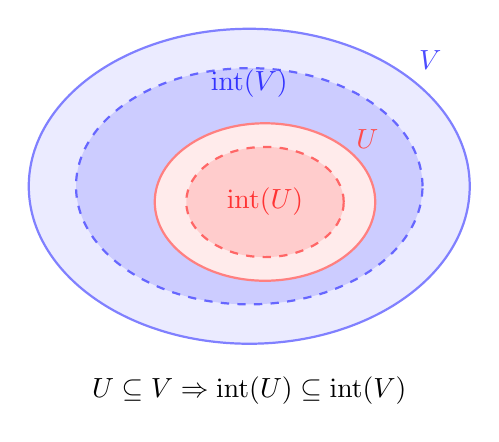
\begin{tikzpicture}[scale=1.0]
  % Outer set V
  \draw[blue!50, fill=blue!8, thick] (0,0) ellipse (2.8cm and 2cm);
  \node[blue!70] at (2.3, 1.6) {$V$};
  % Outer interior V
  \draw[blue!60, fill=blue!20, thick, dashed] (0,0) ellipse (2.2cm and 1.5cm);
  \node[blue!80] at (0, 1.3) {$\inte(V)$};

  % Inner set U
  \draw[red!50, fill=red!8, thick] (0.2, -0.2) ellipse (1.4cm and 1cm);
  \node[red!70] at (1.5, 0.6) {$U$};
  % Inner interior U
  \draw[red!60, fill=red!20, thick, dashed] (0.2, -0.2) ellipse (1cm and 0.7cm);
  \node[red!80] at (0.2, -0.2) {$\inte(U)$};

  % Labels below
  \node at (0, -2.6) {$U \subseteq V \Rightarrow \inte(U) \subseteq \inte(V)$};
\end{tikzpicture}
\caption{内部の単調性: 開集合が大きければ内部も大きい}
\label{fig:interior-monotone}
\end{figure}

\begin{theorem}[内部タワーの特徴付け]
\label{thm:interior-char}
\[
  x \in \mathsf{interiorTower}.\level(U) \;\iff\; U \in \mathcal{N}_x.
\]
すなわち,$\level(U)$ の点は「$U$ が近傍となる点全体」= $\inte(U)$ に一致する。
\end{theorem}

\begin{proofstrategy}
Mathlib の \texttt{mem\_interior\_iff\_mem\_nhds} 補題がこれを直接与える。
\end{proofstrategy}

\begin{leancode}
def interiorTower : StructureTower (Set a) a where
  level U        := interior U
  monotone_level := fun U V hUV => interior_mono hUV

theorem mem_interiorTower_iff (U : Set a) (x : a) :
    x ∈ interiorTower.level U ↔ U ∈ nhds x :=
  mem_interior_iff_mem_nhds
\end{leancode}

\begin{theorem}[開被覆の内部の合併]
\label{thm:interior-union}
開集合族 $\mathcal{U}$ に対して,
\[
  \bigcup_{U \in \mathcal{U}} \inte(U) = \bigcup_{U \in \mathcal{U}} U.
\]
\end{theorem}

\begin{proof}
$(\subseteq)$: $\inte(U) \subseteq U$ は常に成立。
$(\supseteq)$: $U$ が開集合ならば $\inte(U) = U$(開集合は自身の内部に等しい)。
よって等号が成立する。
\end{proof}

\begin{leancode}
theorem interiorTower_iSup_open (U : Set (Set a)) (hopen : forall U ∈ U, IsOpen U) :
    ⋃ U ∈ U, interior U = ⋃ U ∈ U, U := by
  ext x; simp only [Set.mem_iUnion]
  constructor
  · rintro ⟨U, hU, hx⟩; exact ⟨U, hU, interior_subset hx⟩
  · rintro ⟨U, hU, hx⟩; exact ⟨U, hU, (hopen U hU).interior_eq.symm ▸ hx⟩
\end{leancode}

% =============================================================================
\section{三分野の比較}
\label{sec:comparison}
% =============================================================================

StructureTower の真価は,同一の操作($\NatIncl$・$\reindex$・$\iInf$)が
三分野でそれぞれ自然な数学的概念に対応していることにある。

\begin{analogybox}
\begin{center}
\renewcommand{\arraystretch}{1.5}
\begin{tabular}{>{\bfseries}l p{3.2cm} p{3.2cm} p{3.2cm}}
\toprule
操作 & 順序論 & 代数(フィルター)& 位相(内部)\\
\midrule
$\level(i)$ & $(-\infty, x_i]$(下集合)& 部分群 $G_i$ & $\inte(U_i)$\\
$\NatIncl$ & $x_i \leq y_i$(点別)& $F_i \subseteq G_i$ & 位相の細分\\
$\reindex(f)$ & 列の前合成 & 添字群の準同型 & 連続写像の引き戻し\\
$\iInf$ & 下限 & フィルトレーションの交叉 & フィルターの下限\\
\bottomrule
\end{tabular}
\end{center}
\end{analogybox}

\subsection{NatInclusion の位相的意味}

\begin{theorem}[NatInclusion と開集合の包含]
\label{thm:nat-inclusion-interior}
$U_1 \subseteq U_2$ ならば,
定値タワー $\reindex(\mathrm{const}_{U_i})\,\mathsf{interiorTower}$ の間に
$\NatIncl$ が成立する:
\[
  \inte(U_1) \subseteq \inte(U_2).
\]
\end{theorem}

\begin{proofstrategy}
$\reindex(\mathrm{const}_{U_i})$ は単一レベルのタワーを作り,
その包含は $\inte(U_1) \subseteq \inte(U_2)$ に帰着する。
これは Mathlib の \texttt{interior\_mono} が与える。
\end{proofstrategy}

\subsection{reindex の位相的意味: 連続写像の引き戻し}

\begin{theorem}[連続写像と内部タワーの reindex]
\label{thm:reindex-continuous}
連続写像 $f\colon \beta \to \alpha$ と開集合 $U \subseteq \alpha$ に対して,
\[
  f^{-1}(\inte(U)) \subseteq \inte(f^{-1}(U)).
\]
\end{theorem}

\begin{figure}[H]
\centering
\begin{tikzcd}[column sep=4.5em, row sep=3em]
  \beta \arrow[r, "f"] \arrow[d, "{\inte(f^{-1}(U))}"', phantom]
  & \alpha \arrow[d, "{\inte(U)}", phantom] \\
  f^{-1}(\inte(U)) \arrow[r, hook, "f"] \arrow[u, phantom, "\ni" rotate=90]
  & \inte(U) \arrow[u, phantom, "\ni" rotate=90] \\
  f^{-1}(U) \arrow[u, hook, "\subseteq"] \arrow[r, hook, "f"]
  & U \arrow[u, hook, "\subseteq"']
\end{tikzcd}
\caption{連続写像 $f$ による内部タワーの引き戻し}
\label{fig:reindex-continuous}
\end{figure}

\begin{proofstrategy}
Mathlib の \texttt{preimage\_interior\_subset\_interior\_preimage} 補題を適用する。
連続写像は開集合の逆像が開集合という性質から,内部の逆像が逆像の内部に含まれることが従う。
\end{proofstrategy}

\begin{leancode}
theorem reindex_interiorTower_continuous
    {b : Type*} [TopologicalSpace b]
    (f : b -> a) (hf : Continuous f) (U : Set a) :
    f ⁻¹' (interiorTower.level U) ⊆
    interiorTower.level (f ⁻¹' U) := by
  simpa [interiorTower] using
    (preimage_interior_subset_interior_preimage (f := f) (t := U) hf)
\end{leancode}

\subsection{iInf の位相的意味: フィルターの下限}

\begin{theorem}[filterTower の iInf とフィルターの交叉]
\label{thm:iinf-filter}
フィルターの族 $\{F_s\}_{s \in \sigma}$ に対して,
定値タワーの $\iInf$ は各フィルターの集合族の交叉に等しい:
\[
  \left(\iInf_{s \in \sigma}\, \reindex(\mathrm{const}_{F_s})\;\mathsf{filterTower}\right).\level(\star)
  = \bigcap_{s \in \sigma} F_s.\mathrm{sets}.
\]
\end{theorem}

\begin{proofstrategy}
$\iInf$ の定義より $\level(\star) = \bigcap_s \reindex(\mathrm{const}_{F_s}).\level(\star) = \bigcap_s F_s.\mathrm{sets}$。
Lean では \texttt{simp} と定義展開だけで証明できる。
\end{proofstrategy}

\begin{figure}[H]
\centering
\begin{tikzcd}[column sep=3em, row sep=3em]
  \mathsf{filterTower}_{F_1}
    \arrow[dr, phantom, "\bigcap" description, very near start]
  & \mathsf{filterTower}_{F_2} & \cdots & \mathsf{filterTower}_{F_n} \\
  & \iInf_s\, \mathsf{filterTower}_{F_s} \arrow[u, phantom, "\rotatebox{90}{=}"]\\
  & \displaystyle\bigcap_{s} F_s.\mathrm{sets} \arrow[u, equal]
\end{tikzcd}
\caption{iInf によるフィルタータワーの交叉}
\label{fig:iinf-filter}
\end{figure}

% =============================================================================
\section{位相群フィルトレーション}
\label{sec:topgroup}
% =============================================================================

\subsection{類比: 代数 vs. 位相}

FilteredGroup の乗法条件 $G_i \cdot G_j \subseteq G_{i+j}$ と,
位相群の近傍乗法 $U, V \in \mathcal{N}(e) \Rightarrow \exists W \in \mathcal{N}(e),\; W \cdot W \subseteq U \cap V$
は,いずれも「二項演算が添字(または近傍)を保つ」という同型の公理を表す。

\begin{definition}[単位元近傍タワー]
\label{def:unit-nbhd-tower}
位相群 $G$ の単位元 $e$ の近傍系を次で捉える:
\[
  \mathsf{unitNeighborhoodTower}.\level(U)
  \coloniss \{V \in \mathcal{N}(e) \mid V \subseteq U\}.
\]
添字集合は $(\mathcal{P}(G), \subseteq)$(通常の包含順)。
\end{definition}

\begin{figure}[H]
\centering
\begin{tikzcd}[row sep=3em, column sep=5em]
  G_i \times G_j \arrow[r, "\cdot"] \arrow[d, hook, "\subseteq"', "\text{FilteredGroup}"'] & G_{i+j} \\
  \mathcal{N}(e) \times \mathcal{N}(e) \arrow[r, "\cdot"'] \arrow[u, phantom, "\text{vs.}", sloped] & \mathcal{N}(e)
    \arrow[u, phantom]
\end{tikzcd}
\caption{代数(FilteredGroup)と位相群の乗法条件の対応}
\label{fig:topgroup-analogy}
\end{figure}

\begin{theorem}[位相群の近傍乗法定理]
\label{thm:nbhd-mul}
位相群 $G$ において,$U \in \mathcal{N}(e)$ ならば,
\[
  \exists V \in \mathcal{N}(e),\; V \cdot V \subseteq U.
\]
\end{theorem}

\begin{proof}
乗法写像 $\mu\colon G \times G \to G$,$(g, h) \mapsto gh$ は連続であるから,
$e \cdot e = e$ の近傍 $U$ の逆像 $\mu^{-1}(U) \in \mathcal{N}(e, e) = \mathcal{N}(e) \times \mathcal{N}(e)$(積フィルター)。
積フィルターの定義より $V \in \mathcal{N}(e)$ および $W \in \mathcal{N}(e)$ が存在して
$V \times W \subseteq \mu^{-1}(U)$,すなわち $V \cdot W \subseteq U$。
$V \cap W \in \mathcal{N}(e)$ とすれば $(V \cap W) \cdot (V \cap W) \subseteq V \cdot W \subseteq U$。
\end{proof}

\begin{leancode}
theorem unitNeighborhood_mul_property (U : Set G) (hU : U ∈ nhds (1 : G)) :
    ∃ V ∈ nhds (1 : G), V * V ⊆ U := by
  have hUprod : U ∈ nhds ((1 : G) * (1 : G)) := by simpa using hU
  have hmul : Filter.Tendsto (fun p : G × G => p.1 * p.2)
      (nhds ((1 : G), (1 : G))) (nhds ((1 : G) * (1 : G))) := tendsto_mul
  have hpre : {p : G × G | p.1 * p.2 ∈ U} ∈ nhds ((1 : G), (1 : G)) :=
    hmul hUprod
  rw [nhds_prod_eq, Filter.mem_prod_iff] at hpre
  rcases hpre with ⟨V, hV, W, hW, hVW⟩
  refine ⟨V ∩ W, Filter.inter_mem hV hW, ?_⟩
  intro x ⟨v, hv, w, hw, rfl⟩
  exact hVW (show (v, w) ∈ V ×ˢ W from ⟨hv.1, hw.2⟩)
\end{leancode}

\begin{mathinsight}
この定理の証明で重要な役割を果たすのは \texttt{tendsto\_mul}(乗法の連続性)と
\texttt{nhds\_prod\_eq}(積位相での近傍の分解)である。
証明の本質は,連続写像の逆像が近傍を保つという位相の基本性質にある。
\end{mathinsight}

\subsection{単位元近傍タワーの単調性}

\begin{proposition}
$U_1 \subseteq U_2$ ならば $\mathsf{unitNeighborhoodTower}.\level(U_1) \subseteq \level(U_2)$。
\end{proposition}

\begin{proof}
$V \in \level(U_1)$ とすると $V \in \mathcal{N}(e)$ かつ $V \subseteq U_1 \subseteq U_2$。
よって $V \in \level(U_2)$。
\end{proof}

\begin{leancode}
def unitNeighborhoodTower : StructureTower (Set G) (Set G) where
  level U        := {V | V ∈ nhds (1 : G) ∧ V ⊆ U}
  monotone_level := by
    intro U1 U2 hU12 V ⟨hV, hVU1⟩
    exact ⟨hV, Subset.trans hVU1 hU12⟩
\end{leancode}

% =============================================================================
\section{三分野横断 API の全体像}
\label{sec:api-overview}
% =============================================================================

以下の表が「3分野以上で同一 API が効く」昇格条件の証拠をまとめたものである。

\begin{table}[H]
\centering
\renewcommand{\arraystretch}{1.6}
\begin{tabular}{>{\bfseries\sffamily}l p{2.8cm} p{3.0cm} p{3.2cm}}
\toprule
\sffamily\bfseries StructureTower 操作
  & \sffamily\bfseries 順序論
  & \sffamily\bfseries 代数(フィルター)
  & \sffamily\bfseries 位相空間 \\
\midrule
$\level(i)$ & $(-\infty, x_i]$ & 部分群 $G_i$ & $\inte(U_i)$ \\
$\mathsf{monotone\_level}$ & 推移律 & $G_i \subseteq G_j$ $(i \leq j)$ & $U \subseteq V \Rightarrow \inte(U) \subseteq \inte(V)$ \\
$\NatIncl(T_1, T_2)$ & $x_i \leq y_i$ (点別) & $F_i \subseteq G_i$ & 位相の細分 \\
$\reindex(f)$ & 列の前合成 & 添字群の準同型 & 連続写像の引き戻し \\
$\iInf(T_s)$ & 下限 & フィルトレーションの交叉 & フィルターの $\iInf$ \\
$\iSup(T_s)$ & 上限 & 生成されたフィルトレーション & フィルターの $\iSup$ \\
乗法条件 & (なし)& $G_i \cdot G_j \subseteq G_{i+j}$ & $V \cdot V \subseteq U$ ($V \in \mathcal{N}(e)$) \\
\bottomrule
\end{tabular}
\caption{StructureTower API の三分野における意味の対応表}
\label{tab:comparison}
\end{table}

\begin{figure}[H]
\centering
\begin{tikzcd}[column sep=2.5em, row sep=3.5em, every arrow/.style={-Latex}]
  & \mathsf{StructureTower}(\iota, \alpha) \arrow[dl, bend right=10, "\text{フィルター添字}"'] \arrow[d, "\text{開集合添字}"] \arrow[dr, bend left=10, "\text{位相群添字}"] &\\
  \mathsf{filterTower} \arrow[drr, dashed, bend right=15, "\iInf"']
  & \mathsf{openCoverTower} \arrow[dr, dashed, "\reindex"]
  & \mathsf{unitNbhdTower} \\
  & & \mathsf{interiorTower} \arrow[ul, phantom, "\simeq" description]
\end{tikzcd}
\caption{三分野のタワーと StructureTower 操作の関係図}
\label{fig:api-diagram}
\end{figure}

% =============================================================================
\section{型検査による検証}
\label{sec:typecheck}
% =============================================================================

Lean~4 の型検査器は,各タワーが正しく \texttt{StructureTower} の形を持つことを保証する。

\begin{leancode}
-- 順序論タワー: StructureTower a a(Iic 塔)
example [Preorder a] : StructureTower a a where
  level x        := Set.Iic x
  monotone_level := fun _i _j hij _y hy => le_trans hy hij

-- 位相タワー: StructureTower (Set a) a
example : StructureTower (Set a) a := interiorTower

-- 位相群タワー: StructureTower (Set G) (Set G)
example : StructureTower (Set G) (Set G) := unitNeighborhoodTower
\end{leancode}

これらの \texttt{example} 宣言が Lean にエラーなく受理されることが,
「代数・順序・位相の三分野が同一の API で記述できる」ことの形式的な証拠である。

% =============================================================================
\section{まとめと展望}
\label{sec:conclusion}
% =============================================================================

本稿では,Lean~4 / Mathlib4 における \texttt{StructureTower} という抽象的な概念を用いて,
位相空間論の中核的な対象——フィルター・開被覆・内部作用素——を統一的に記述した。

\medskip

\textbf{達成したこと:}
\begin{itemize}
  \item \texttt{StructureTower} のコア定義と三つの基本操作($\NatIncl$・$\reindex$・$\iInf$)の Lean 実装
  \item 位相空間向けの四種のタワー構造(近傍タワー・フィルタータワー・開被覆タワー・内部タワー)の構築
  \item 連続写像の引き戻しと内部タワーの対応(\cref{thm:reindex-continuous})
  \item 位相群における FilteredGroup との類比の形式化(\cref{thm:nbhd-mul})
  \item 型検査による三分野横断性の形式的検証
\end{itemize}

\medskip

\textbf{今後の展開:}
\begin{itemize}
  \item 一様空間(uniform spaces)への拡張: 近縁系(entourages)を
    StructureTower の添字として捉えることができるか
  \item 圏論的定式化: StructureTower の自然変換として $\NatIncl$ を捉え,
    関手圏での $\iInf$・$\iSup$ との対応を見る
  \item 完備化との接続: Cauchy フィルターの極限が
    StructureTower のどのような収束概念に対応するか
  \item 代数幾何への展開: スキームの位相とフィルトレーションの統一的記述
\end{itemize}

\begin{mathinsight}
StructureTower の本質的な力は,「型が合う」という Lean の検査が
「数学的に同じ構造である」という洞察を自動的に保証する点にある。
三分野で同じ API を使えることは,それらが本質的に同じ構造の異なる顔であることを
機械的に証明している。
\end{mathinsight}

% =============================================================================
\end{document}
